\documentclass[../../main.tex]{subfiles}

% 

\begin{document}
\chapter{Zdroje částic}

\section{Přehled}

Částice vznikají v rozpadu - využívají se při kalibraci detektorů ale i při výzkumu a aplikacích (lékařské, materiálové, ...)

Sekundární částice vznikají v reakcích s využitím urychlovačů - s vysokou energií

Zdroje elektronů:
\begin{itemize}
	\item rozpad beta (spojité spektrum)
	\item konverzní elektrony (diskrétní spektrum)
\end{itemize} 

Příklady zdrojů elektronů z rozpadu beta:
\begin{center}
	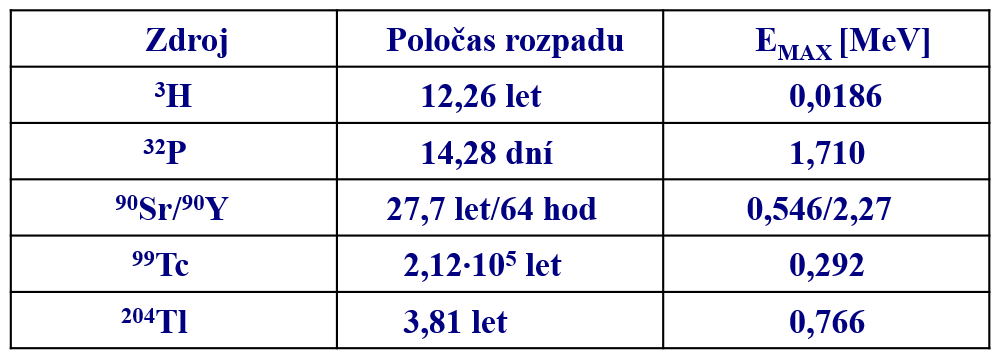
\includegraphics[width=0.6\textwidth]{elektrony.png}
	\captionof{figure}{Příklady zdrojů elektronů z rozpadu beta}		
\end{center}

Zdroje alfa:
\begin{itemize}
	\item rozpad alfa (diskrétní spektra)
	\item jaderné reakce (diskrétní spektrum)
\end{itemize}

Příklady zdrojů částic alfa z rozpadu:
\begin{center}
	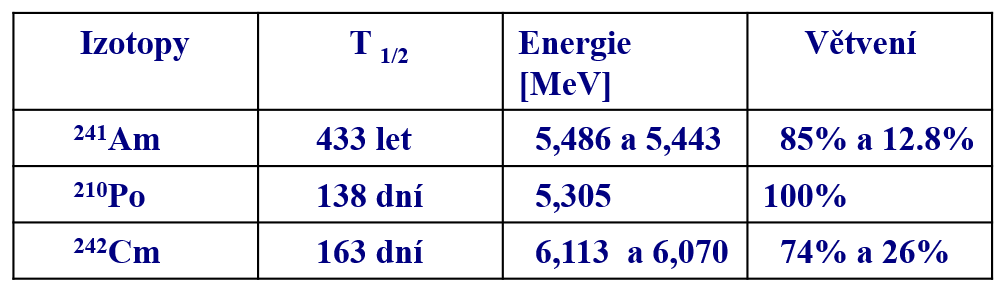
\includegraphics[width=0.6\textwidth]{alfa3.png}
	\captionof{figure}{Příklady zdrojů částic alfa z rozpadu}		
\end{center}

Náboj částic alfa je $Z=2$ $\rightarrow$ vysoké energetické ztráty a absorbce při průchodu hmotou $\rightarrow$ zdroje alfa se dávají na podložku a překrývají se extrémně tenkou kovovou fólií

Zdroje záření gamma:
\begin{itemize}
	\item Rozpad gamma následující rozpad beta (diskrétní spektrum)
	\item Záření vznikající při anihilaci pozitronu $E_{\gamma} = 511 ~\mathrm{keV}$
	\item Brzdné záření
\end{itemize}

Příklady zdrojů záření gamma:
\begin{center}
	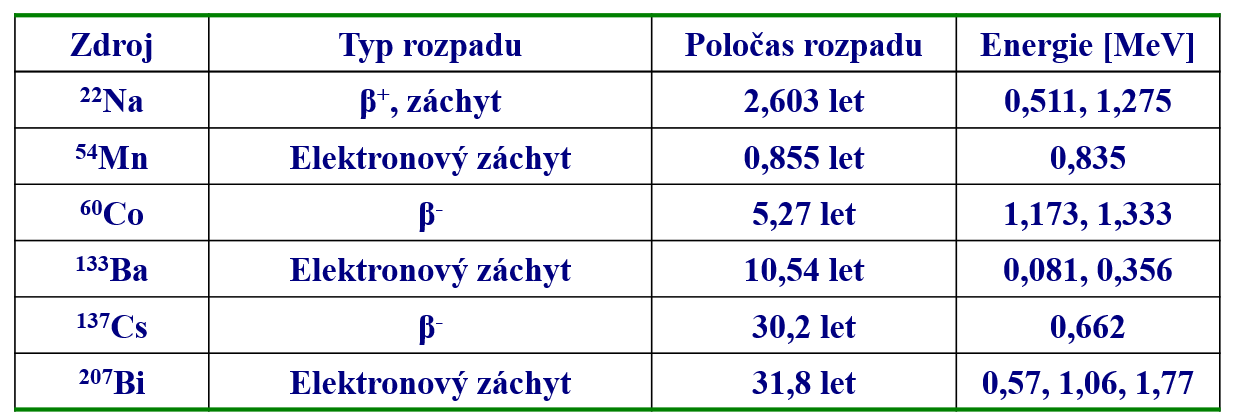
\includegraphics[width=0.6\textwidth]{gamma2.png}
	\captionof{figure}{Příklady zdrojů záření gamma}		
\end{center}

Neutronové zdroje:
\begin{itemize}
      \item Spontánní štěpení jader
      \item Štěpení jader, jaderné reaktory
      \item Jaderné reakce - spojení rozpadu alfa a reakce ($\alpha$, n), rozpadu gamma a reakce ($\gamma$, n) reakce urychlených protonů na lehkém terči, např. na lithiu, beryliu, deuteriu
      \item Tříštivé reakce relativistických protonů s těžkými jádry 
\end{itemize}

Příklady neutronových zdrojů využívající reakce:

Většinou zdroj alfa a $Be$: $Pu+Be$, $Am+Be$

Zdroj jader (radioaktivních):
\begin{itemize}
	\item štěpení jader - spontánní i indukované
	\item jaderné reakce
	\item tříštivé reakce
\end{itemize}

Zdroje iontů (pro další urychlení)

Zdroje antičástic, podivných baryonů, mezonů, mionů, tauonů ... - využití urychlovačů a reakcí vysokoenergetických částic s terči

Zdroj ultrarelativistických částic s minimální ionizací (mionů) - kosmické záření

\section{Zdroje elektronů}

\subsection{Beta rozpad}

Nejčastěji využívaným zdrojem rychlých elektronů bývají radioizotopy rozpadající se $\beta ^-$ přechodem
\begin{equation}
^{A}_{Z}X \rightarrow ^{A}_{Z+1}Y + e^- + \bar{\nu _e},
\end{equation}
kde $X$ je mateřské jádro a $Y$ je dceřiné jádro a $\bar{\nu _e}$ elektronové antineutrino. Vzhledem k velmi malé pravděpodobnosti interakce neutrin s látkou zde nemusíme detekci těchto částic uvažovat. Dceřinné jádro $Y$ obdrží při rozpadu velmi malou energii, která je běžně pod prahem ionizace. Jediným podstatným producentem ionizujícího záření při beta přechodech je tak elektron. 

Většina radionuklidů produkovaných srážkami neutronů se stabilními prvkami je beta radioaktivní, je tak možno vytvořit velké množství beta záření emitujících nuklidů s poločasy rozpadu od tisíců let až po poločasy, které lze prakticky využít. Při beta přechodu je dceřinné jádro obvykle ponecháno v některém z excitovaných stavů, ze kterého přechází do základního následnou emisí gamma záření, které doprovází emitovaný elektron z beta rozpadu. Několik příkladů nuklidů, které přecházejí přímo do základního stavu dceřinného jádra a jsou tak producenty čistého beta záření, je uvedeno v tabulce.

\begin{center}
	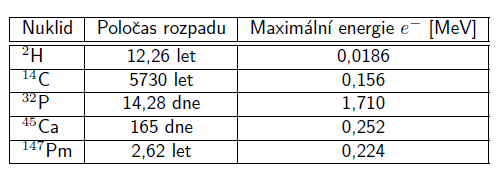
\includegraphics[width=0.6\textwidth]{nuklidy.png}
	\captionof{figure}{Příklady producentů čistého beta záření}		
\end{center}

Každý beta rozpad je charakterizován pevně danou energií přechodu $Q$, která se dělí mezi elektron a neutrino. Energie elektronu se tak může lišit případ od případu a může nabývat od nulové hodnoty až po maximální energii , která je numericky rovna energii přechodu $Q$.  

\subsection{Vnitřní konverze}

Spojité spektrum energií elektronů produkovaných beta zářiči je pro některé aplikace nevhodné. Naproti tomu proces vnitřní konverze může za jistých podmínek poskytnout téměř monoenergetické elektrony. 

K vnitřní konverzi dochází, je-li jádro produkováno v excitovaném stavu, ze kterého nepřejde do základního stavu běžnou emisí gamma kvanta, ale předá svou excitační energii $E_{ex}$ jednomu z orbitálních elektronů, který je následně uvolněn s energií

\begin{equation}
E_e = E_{ex} - E_b,
\end{equation} 
kde $E_b$ je vazebná energie elektronu ve slupce, ve které se nachází. 

Konverzní elektron může pocházet z jakékoliv slupky (je-li jeho emise na dané slupce energeticky možná). Jedna excitovaná hladina atomového jádra tak může vést k emisi několika skupin elektronů o různých energiích. Další komplikace nastávají v případech, kdy jsou ve zdroji záření jádra v různých excitovaných stavech. Spektrum konverzních elektronů se navíc vždy skládá se spojitým spektrem elektronů, které byly emitovány při rozpadu mateřského jádra. 

\begin{center}
	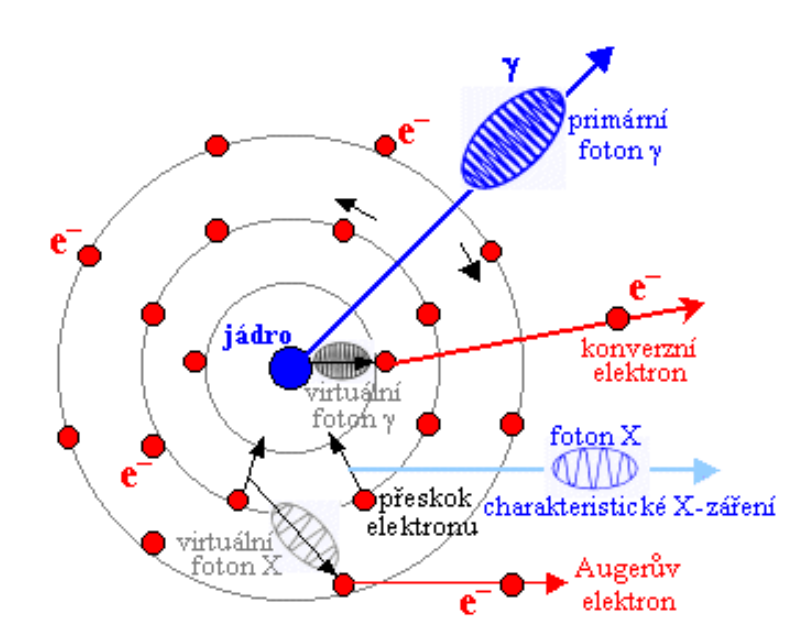
\includegraphics[width=0.8\textwidth]{auger_2.png}
	\captionof{figure}{Vnitřní konverze}		
\end{center}  

\subsection{Augerovy elektrony}
 
 Augerovy elektrony jsou přibližně vzato analog konverzních elektronů v případech, kdy excitační energie "pochází" z celého atomu. Existují procesy, při kterých v atomovém obalu vznikne vakance v některé elektronové slupce. Běžně je tato vakance zaplněna eelktronem z některé vyšší slupky, přičemž je emitováno gamma kvantum odnášející energii rovnou rozdílu energií daných elektronových slupek.
 
 Tato excitační energie atomu však může být alternativně předána jednomu z vnějších elektronů, který následně opouští atom. Tento elektron se nazývá Augerův a nese energii, která odpovídá rozdílu energií mezi původní excitační energií atomu a vazebnou energií slupky, na které se nacházel. Augerovy elektrony tak mají DISKRÉTNÍ ENERGETICKÉ SPEKTRUM. Jejich energie jsou ve srovnání s předešlými způsoby produkce elektronů malé, neboť emise Augerových elektronů je upřednostňována v prvcích s malým $Z$, pro které je elektronová vazebná energie malá.
 
 Ačkoli tento jev objevila r. 1923 Lise Meitnerová, pojmenován byl po Pierru Augerovi, který ho dva roky poté znovuobjevil. 
 
 \begin{center}
 	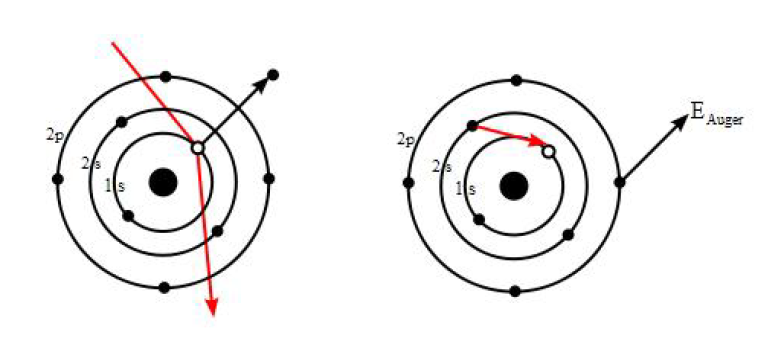
\includegraphics[width=0.8\textwidth]{auger.png}
 	\captionof{figure}{Augerovy elektrony}		
 \end{center}  
 
\section{Zdroje těžkých nabitých částic}

\subsection{Alfa rozpad}

Těžká jádra jsou energeticky nestabilní vůči spontánní emisi alfa částice. Pravděpodobnost rozpadu je řízena mechanismem penetrací Coulombické bariéry jádra. Poločas rozpadu vhodných zdrojů je v rozsahu od dnů po spousty tisíc let. 

Alfa částice se vyskytují v jedné či několika energetických skupinách, které jsou vždy monoenergetické. Každý přechod mezi mateřským a dceřiným (tj. mezi základním stavem mateřského jádra a základním stavem dceřinného jádra) charakterizuje hodnota $Q$ udávající energetický rozdíl mezi počátečním a koncovým stavem. tato energie se jednoznačným způsobem dělí mezi alfa částici a odražené jádro, a tudíž si každá alfa částice odnáší energii
\begin{equation}
T_{\alpha} = \dfrac{A-4}{A} Q.
\end{equation} 

Je mnoho případů. kde se mezi mateřským a dceřinným jádrem uděje pouze jeden přechod a kdy je tedy alfa částice emitována s jednoznačně danou energií. Pokud je možný přechod na více hladin dceřinného jádra, může energie alfa částice nabývat více hodnot. 

Většina alfa částic má energii od 4 po 6$\mathrm{MeV}$. Navíc existuje silná závislost mezi energií alfa částice a poločasem rozpadu daného mateřského jádra - čím vyšší energie alfa částice, tím kratší poločas rozpadu. Přibližně pod $6,5 ~\mathrm{Mev}$ bývá poločas rozpadu menší než několik dnů, tyto zdroje mají tudíž menší užitek. Na druhou stranu při poklesu energie pod $4 ~\mathrm{MeV}$ se stane pravděpodobnost průchodu alfa částice Coulombovskou bariérou velmi malou a poločas rozpadu mateřského jádra tedy velmi vzroste. 

Jelikož alfa částice při průchodu materiálem ztrácí svou energii velmi rychle, aby jejich zdroje byly monoenergetické, je třeba je připravovat ve velmi tenkých vrstvách.

\begin{figure}[h!]
	\begin{minipage}[c]{0.55\linewidth}
		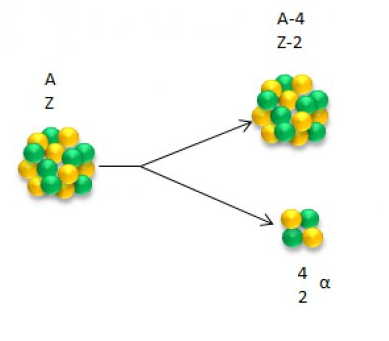
\includegraphics[width=\linewidth]{alfa.png}
	\end{minipage}
	\hfill
	\begin{minipage}[c]{0.55\linewidth}
		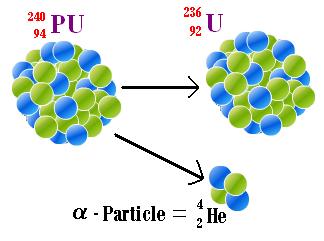
\includegraphics[width=\linewidth]{alfa2.png}
	\end{minipage}
	\caption{Alfa rozpad}
\end{figure}

\subsection{Spontánní štěpení}

Štěpný proces je jediným spontánním zdrojem energetických těžkých nabitých částic s hmotou větší než alfa částice. Štěpné produkty jsou tudíž široce využívané při kalibraci a testování detektorů určených k měření ve fyzice těžkých iontů. 

Všechna těžká jádra jsou v principu nestabilní vůči spontánnímu štěpení na dvě lehčí jádra. Vzhledem k tomu, že jádra při tomto procesu musí překonávat velké potenciálové bariéry nutné k roztržení jádra z jeho původně téměř sférického tvaru, děje se tento proces zejména u extrémně těžkých jader - transuranových izotopů s velkým hmotovým číslem. Nejvíce využívaným příkladem je kalifornium $^{252}Cf$, které podléhá spontánnímu štěpení s poločasem 85 let a které navíc při každém štěpení uvolní spoustu rychlých neutronů (většina transuranů ovšem podléhá také alfa rozpadu, jehož pravděpodobnost je mnohem vyšší).

Při každém štěpení vznikají dva fragmenty (odštěpky), které díky zákonu zachování hybnosti jsou emitovány v opačných směrech. Jelikož zdroj spontánního štěpení je převážně asymetrické, jsou fragmenty shlukovány do lehké skupiny a těžké skupiny s průměrnými hmotovými čísly 108 a 143. Původně jsou fragmenty kladnými ionty, avšak zpomalováním interakcemi s látkou, kterou prochází, snadno  naberou elektrony, které redukují jejich efektivní náboj. Průměrná energie rozdělená mezi dva fragmenty činí 185 $\mathrm{MeV}$, její rozdělení je opět asymetrické s tím, že lehčí fragment si odnáší větší díl. 

Jelikož štěpné fragmenty velmi ochotně ztrácejí energii při průchodu látkou, pokud není zdroj připraven ve formě velmi tenké desky, je třeba při jejich produkci počítat se samoabsorbcí v materiálu či s podstatnými energetickými ztrátami.  

 \begin{center}
	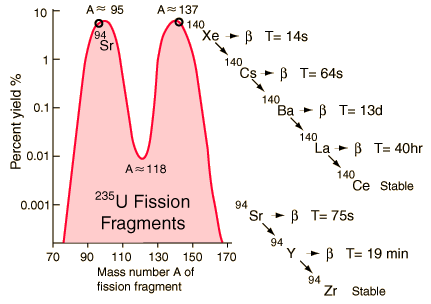
\includegraphics[width=0.7\textwidth]{step.png}
	\captionof{figure}{Štěpení uranu}		
\end{center} 

\section{Zdroje neutronů}

Zdroje neutronů lze dělit podle způsobu produkce na radioizotopické zdroje, spalační zdroje; neutrony lze také získávat jadernými reakcemi pomocí urychlovačů i reaktorů (neutrony indukované štěpení).

Důležité je rozdělení neutronů podle kinetické energie, kde nás zajímají zejména tepelné neutrony.

 \begin{center}
	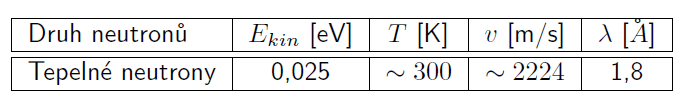
\includegraphics[width=0.8\textwidth]{neutr.png}
	\captionof{figure}{Vlastnosti tepelných neutronů}		
\end{center}

\subsection{Radioizotopické neutronové zdroje}

Přímé radioizotopické zdroje neutronů prakticky nejsou dostupné; pouze $^{8}Be$ se specifickým $\beta$ rozpadem , který vede k excitovanému stavu, jenž se dále rozpadá emisí neutronů, je využitelný.

Mohou se však využít fotoneutronové zdroje - ty jsou založeny na absorbci fotonu, jenž vede k následné emisi neutronu. Platí, že monoenergetické fotony produkují přibližně monoenergetické neutrony. Pro produkci neutronů o smysluplné intenzitě jsou zapotřebí velké intenzity fotonů - pouze přibližně jeden foton z $10^5$ až $10^6$ fotonů generuje neutron.

Dvě reakce jsou zde využitelné:
\begin{equation}
\gamma  + ^{9}Be \rightarrow ^{8}Be + n, ~~~~~~ Q = - 1,666 ~\mathrm{MeV},
\end{equation} 
\begin{equation}
\gamma + ^{2}H \rightarrow ^{1}H + n, ~~~~~~ Q = - 2,226 ~\mathrm{MeV}.
\end{equation}

Pro zdroj neutronů lze využít i $\alpha$ částice z přímého $\alpha$ rozpadu několika vhodných radionuklidů. Množství materiálů může vést k reakci ($\alpha$, n) při energiích $\alpha$ částic dostupných z radioaktivního rozpadu. Největšího výtěžku je ale dosáhnuto při volbě berylia za terčíkový materiál (berylium má malou vazebnou energii neutronů $B E_n \approx 1,7 ~\mathrm{MeV}$):
\begin{equation}
\alpha + ^{9}Be \rightarrow ^{12}C + n , ~~~~~~ Q = + 5,7 ~\mathrm{MeV}.
\end{equation}   

Většinou ale s beryliem reaguje pouze $10^{-4}$ $\alpha$ částic; některé vzniklé izotopy mohou vést k velmi dlouhým řetězcům přeměn, které sice přispívají k celkovému výtěžku neutronů, ale také tvoří fotonové pozadí.

\subsection{Neutrony produkované v reakcích s nabitými částicemi}

Spousta jaderných reakcí dokáže produkovat neutrony, nicméně je přitom vyžadován již urychlený svazek částic. Tyto reakce tak nejsou tolik vhodné jako radioaktivní zdroje. Na druhou stranu výběrem vhodné  energie a úhlu nalétávajících částic je možno dosáhnout libovolné energie svazku neutronů, který je navíc monoenergetický. 

\subsection{Spalační neutronové zdroje}

Spalační neutronové zdroje sestávají z urychlovače, jenž poskytuje svazek protonů nebo těžších iontů o dostatečně vysoké energii ($\sim 1 ~\mathrm{GeV}$) a intenzitě, a vhodného terčového materiálu složeného z těžkých jader. Samotná spalační energie, jak je známa ze studií kosmického záření, spočívá ve vyrážení nukleonů z jádra pomocí vysoce energetických bombardujících částic.

Pulsy neutronů z terčového materiálu jsou následně zpomalovány v moderátoru a vedeny dále k detektorům apod.

Urychlovače přitom musí poskytovat velmi krátké pulsy ($< 1 ~\mathrm{ms}$) částic o energii 1 až 3 $\mathrm{GeV}$ s frekvencí $\sim 60 ~\mathrm{Hz}$ k maximalizaci neutronového výtěžku.

\subsection{Spontánní štěpení}

Spontánní štěpení je druhem radioaktivního rozpadu velmi těžkých izotopů (teoreticky možné pro jádra těžší neř 100 $\mathrm{amu}$, energeticky pro jádra těžší než 230 $\mathrm{amu}$). Pro uran a thorium je sice takové štěpení možné, ale jelikož k němu dochází jen ve velmi malé míře, většinou není bráno v potaz.

Ke spontánnímu štěpení zato velmi často ve srovnání s dříve uvedenými prvky dochází u kalifornia $^{252}Cf$, což je transuranový prvek objevený při bombardování curia $\alpha$ částicemi. Je to zároveň nejtěžší prvek, jehož bylo vyprodukováno vážitelné množství. Energie neutronů ze spontánního štěpení kalifornia má spojité rozdělení s průměrnou energií 1 - 3 $\mathrm{MeV}$.
	
Kalifornia se používá jako zdroje neutronů pro nastartování jaderných reaktorů, léčbu nádorů, radiografii, či jako neutronového aktivačního detektoru. Ve vojenství se používá zejména izotop $^{251}Cf$ díky tomu, že má velmi malou kritickou hmotnost (asi 2 $\mathrm{kg}$), vysokou letalitu a s tím spojenou krátkou dobu toxického ozáření.

Matematická podmínka pro to, u kterých prvků může ke spontánnímu štěpení dojít, zní
\begin{equation}
\dfrac{Z^2}{A} \geq 45,
\end{equation}	
kde $Z$ je protonové číslo a $A$ nukleonové číslo.

\section{Zdroje záření $\gamma$}

\subsection{Gamma přechody následující beta rozpad}

Záření gamma je emitováno excitovanými jádry při jejich přechodu k níže ležícím hladinám. U většiny praktických laboratorních zdrojů jsou tyto excitované stavy jader vytvořeny při rozpadu mateřského jádra. 

Čtyři příklady široce používané jako kalibrace zdrojů gamma záření jsou na obrázku. V každém z uvedených případů je excitovaný stav dceřinného jádra vytvořen některým z druhů beta rozpadu, který je ve srovnání s přechodem gamma do základního stavu jádra (typicky v řádech pikosekund či ještě méně) poměrně pomalým procesem charakterizovaným poločasem rozpadu stovky dnů nebo delším. 

\begin{center}
	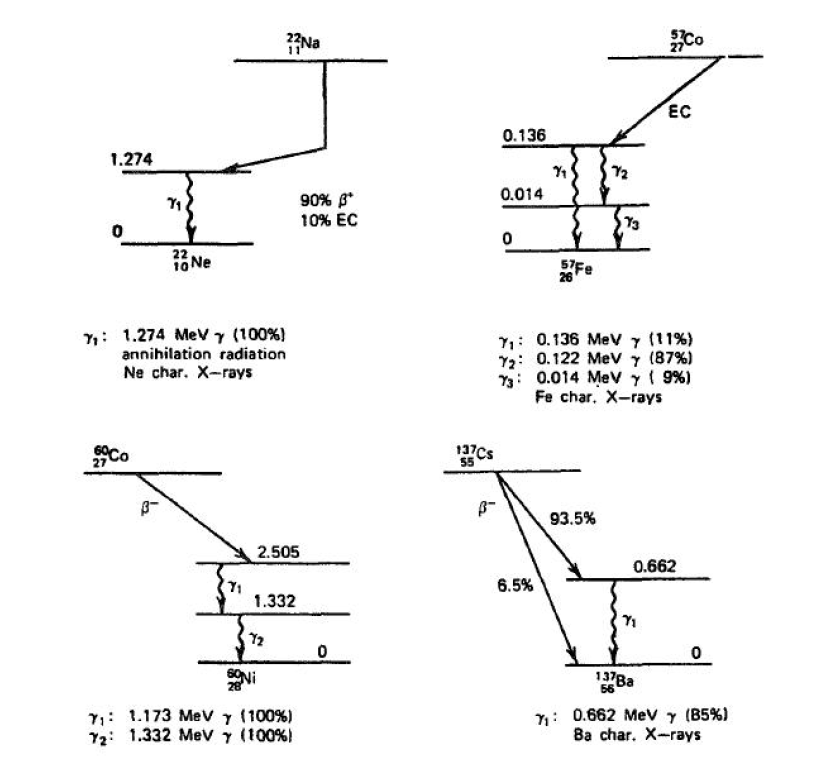
\includegraphics[width=0.8\textwidth]{schem.png}
	\captionof{figure}{Rozpadová schémata pro zdroje gamma záření}		
\end{center}

Deexcitace dceřinného jádra do základního stavu se děje pomocí emise fotonu, jehož energie je přesněrovna rozdílu energií mezi počátečním a koncovým stavem jádra. Záření gamma tak přesně reflektuje strukturu energetických úrovní dceřinného jádra. Jelikož jaderné stavy mají přesně definované energie, jsou energie gamma záření emitované při těchto přechodech také přesně dány a jsou takřka monoenergetické. 

Běžně užívané zdroje gamma záření založené na beta rozpadu jsou limitovány do energií pod $2,8 ~\mathrm{MeV}$. Jediný nuklid, který může sloužit jako potenciální zdroj gamma záření o vyšší energii, je $^{56}Co$. Krátkýpoločas rozpadu (77 dnů) u něj ale limituje použití pouze na zařízení s přístupem k urychlovačům potřebným k jeho produkci skrze reakci $^{56}Fe(p,n)$. Dalším možným radioizotopem pro vysokoeenrgetické kalibrace je $^{16}N$ s energiemi emitovaného gamma záření $6,13$ a $7,11$ $\mathrm{MeV}$ emitovaných při $\beta^-$ přechodu na $^{16}O$. 

Zdroje záření gamma obvykle sestávají ze vzorku radioizotopu ( o aktivitě $10^5 ~\mathrm{Bq}$) uzavřeného v plastovém disku. Tloušťka pouzdra se volí dostatečná , aby zastavila jakékoliv primární částice produkované při beta přechodu a propustila pouze žádané gamma záření.

\subsection{Vyzařování při anihilaci}

Při samovolném $\beta^+$ přechodu je generováno také elektromagnetické záření. Jeho původ spočívá v osudu positronů emitovaných při rozpadu , které procestují látkou pouze několik milimetrů, než ztratí svou kinetickou energii. V případě, že jejich energie je již velmi malá (což je na konci jejich dosahu) anihilují s elektrony vyskytujícími se ve stínícím materiálu. Původní elektron a pozitron zmizí a jsou nahrazeny dvěma opačně směrovanými fotony, z nichž každý má energii 511 $\mathrm{keV}$.

Toto záření se samozřejmě skládá s následujícím zářením emitovaným při přechodu dceřinného jádra do základního stavu. Například v přechodu $^{22}Na$ jsou tímto způsobem emitovány fotony o energiích 511 $\mathrm{keV}$ a 1274 $\mathrm{kev}$ .

\subsection{Záření gamma následující jaderné reakce}

Pakliže je potřeba záření gamma o energiích vyšších, než které jsou dostupné z beta aktivních izotopů, musí se uvážit jiné procesy vedoucí k výše ležícím excitovaným stavům jádra. Jednou z možností je jaderná reakce
\begin{equation}
^{4}_{2}\alpha + ^{9}_{4}Be \rightarrow ^{12}_{6}C^* + n,
\end{equation}
při které je jádro $^{12}C$ ponecháno v excitovaném stavu. Jeho rozpad následně vede k fotonu gamma záření o energii 4,44 $\mathrm{MeV}.$ Naneštěstí jsou průměrné doby života tohoto stavu velice krátké (61 $\mathrm{fs}$), a uhlíkový atom se nestihne před emisí gamma záření uklidnit. Výsledná energie gamma je tak rozmazána Dopplerovskými efekty závisejícími na relativní orientaci odraženého jádra a fotonu; toto rozmazání představuje okolo jednoho procenta energie gamma. Tato šířka je dostačující pro kalibrační účely, ale je příliš velká pro detektory s velmi přesným energetickým rozlišením.

Jinou možností je použití relace
\begin{equation}
^{4}_{2}\alpha + ^{13}_{6}C \rightarrow ^{16}_{8}O^* + n,
\end{equation}
kde se jádro kyslíku formuje ve vzbuzeném stavu 6,13 $\mathrm{MeV}$ nad základním stavem a s dobou života $2\times10^{-11} ~\mathrm{s}$, která je dostatečně dlouhá k eliminaci Dopplerovských efektů. Výsledné záření gamma je tak v podstatě monoenergetické. 

Jelikož většina alfa částic nevede k reakci, dokud neztratí část své energie v terčovém materiálu, je třeba k vytvoření zdroje gamma záření použít radiátor alfa záření o velké aktivitě.

Záření gamma je také vysíláno po absorbci termálních neutronů jádry. Zdroje termálních neutronů zde mohou být intenzivní svazky z jaderných reaktorů či urychlovacích zařízení. U těchto zdrojů gamma se energie záření pohybují až do 9 $\mathrm{MeV}$. 
 
\begin{center}
 	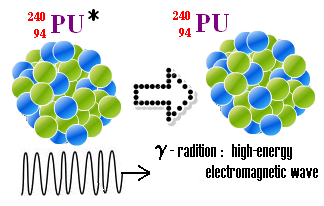
\includegraphics[width=0.6\textwidth]{gamma.png}
 	\captionof{figure}{Vznik gamma záření po přechodu excitovaného jádra do základního stavu}		
\end{center}

\subsection{Brzdné záření} 

Při interakci rychlých elektronů s látkou se část jejich energie mění v elektromagnetické záření ve formě brzdného záření. Část energie elektronu konvertovaná v brzdné záření roste s rostoucí energií elektronu a je největší pro absorbující materiály s vysokým atomovým číslem. Tento proces je důležitý pro produkci rentgenovského záření z konvenčních rentgenek. 

Pro monoenergetické elektrony, které se zpomalí a zastaví v daném materiálu, je spektrum brzdného záření SPOJITÉ s energiemi emitovaných fotonů rostoucími až po původní energii elektronu, přičemž dominuje emise nízkoenergetických fotonů ( do 1/3 energie elektronu) a průměrná energie fotonu je malý zlomek energie elektronu (kolem 1/8 energie elektronu). Střední energie brzdného záření je tedy podstatně nižší než původní energie elektronů.

Jelikož jsou tato spektra spojitá, nelze je použít přímo ke kalibraci detektorů. Tvar spektra lze však měnit použitím různých materiálů, jimiž elektrony prochází.

 \begin{center}
 	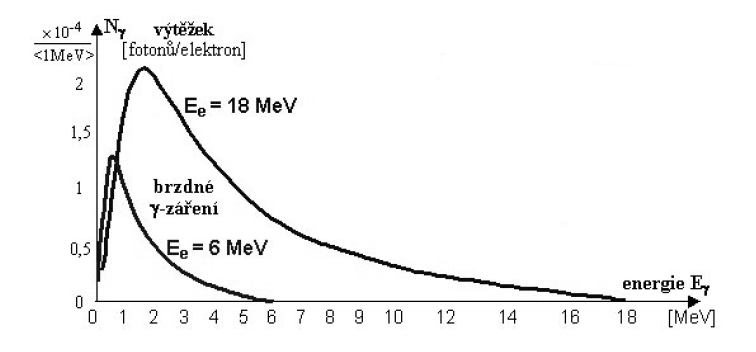
\includegraphics[width=1\textwidth]{brzdne.png}
 	\captionof{figure}{Spektrum brzdného záření vznikajícího dopadem elektronů o energii 6 a 18 $\mathrm{MeV}$}		
 \end{center} 

\subsection{Zdroje částic - Petráček}
\begin{itemize}
	
	\item ZDROJE ELEKTRONŮ
	
	Zdroje elektronů dělíme na diodové a triodové. Výhodou triodových zdrojů je možnost produkovat kratší pulsy s většími proudy svazku. Toho je dosaženo zejména díky tomu, že jsou omezeny kapacity, které je třeba nabíjet na vysoké napětí.
	
	Jako první probereme konstrukci diodového zdroje. Na základě externího signálu dojde k sepnutí elektronky v důsledku čehož vznikne na soustavě LC členů zapojených v jejím anodovém obvodu ke vzniku krátkého vysokonapěťového pulzu. Ten je přiveden koaxiálním kabelem do tělesa samotného zdroje. Tam dojde k transformaci na cca 10x vyšší napětí, které je přivedeno na nepřímo žhavenou katodu emitující elektrony. Tyto elektrony jsou napětím pulsu urychleny a skrze Pierceovu čočku vstříknuty do svazkové trubice.
	
	 \begin{center}
		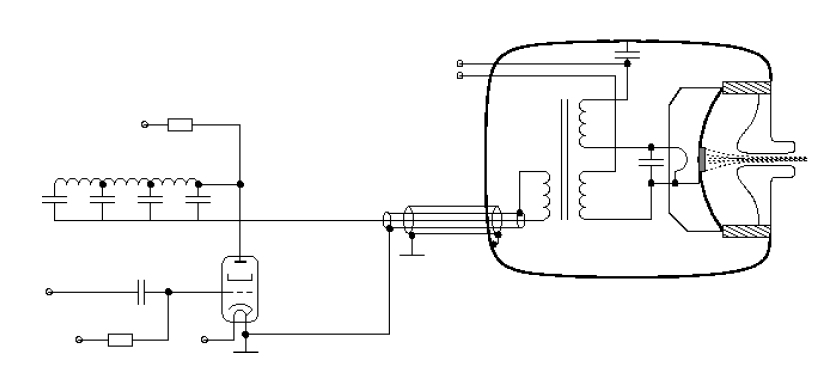
\includegraphics[width=0.7\textwidth]{diod.png}
		\captionof{figure}{Schéma diodového zdroje elektronů}		
	\end{center} 
	
	Katoda musí být žhavená vláknem tak, aby emitovala dostatečné množství elektronů. Těleso zdroje je naplněno transformátorovým olejem, který zabraňuje výbojům v obvodu vysokonapěťového transformátoru. Limitujícím faktorem pro dosažení krátkého pulsu je kapacita koaxiálního vedení, po kterém je veden primární puls o amplitudě cca 5 $\mathrm{keV}$. Aby bylo možno vytvářet pulsy kratší, je třeba pracovat s menší amplitudou pulsu a s co nejmenšími kapacitami. Těmto požadavkům vyhovuje triodový zdroj zobrazený na obrázku. 
	
	Triodový zdroj je stále na vysokém záporném potenciálu přibližně 50 $\mathrm{keV}$. Jeho nepřímo žhavená katoda produkuje stále proud elektronů, ale tento proud nemůže projít přes mřížku polarizovanou tak, že elektrony zastaví. Pouze krátký puls vytvořený v koaxiálním zpožďovacím vedení po sepnutí tranzistoru tuto mřížku otevře a elektrony mohou být urychleny a vstříknuty do svazkové trubice. Spouštěcí impulz musí být do zdroje přiveden pomocí optického kabelu. 
	
	
	\begin{center}
		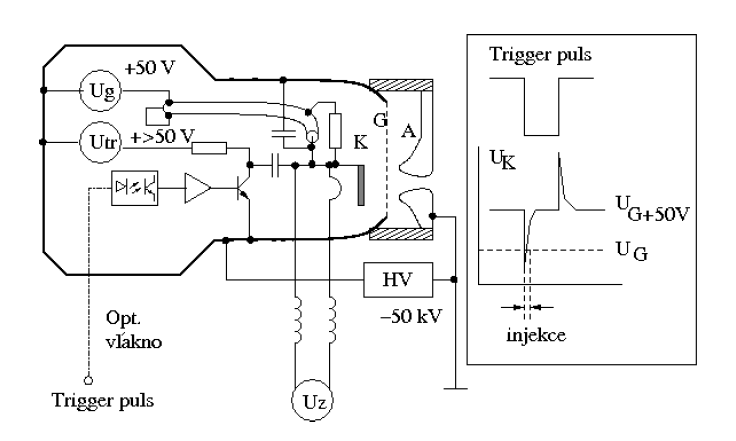
\includegraphics[width=0.7\textwidth]{triod.png}
		\captionof{figure}{Schéma triodového zdroje elektronů}		
	\end{center}
	
	\item ZDROJE POZITRONŮ
	
	Jako zdroj pozitronů lze využít buď $\beta^+$ zdroj (například $^{22}Na$) s moderátorem pozitronů (pevný Xeon) a pozitronovým akumulátorem, nebo lze pozitrony vyrábět procesem tvorby párů $e^+ e^-$. První zmíněný postup se využívá při přípravě velmi chladných pozitronů pro produkci antivodíku, druhý pak při produkci pozitronů pro další urychlení. Wolframový terč je bombardován elektronovým svazkem o energii  $\approx 200 ~\mathrm{MeV}$. Při brždění elektronů vzniká brzdné záření, jehož fotony způsobují v blízkosti wolframových jader tvorbu $e^+ e^- $ párů. Vyletující pozitrony lze vyfiltrovat z reakčních produktů pomocí magnetického pole. Vznikající pozitrony mají široké spektrum energií sahajících až do 30 $\mathrm{MeV}$.
	
	
	\begin{center}
		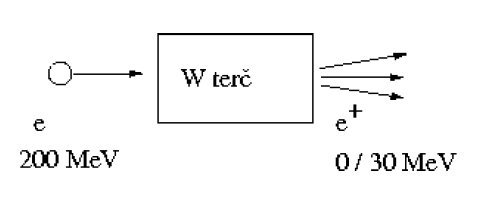
\includegraphics[width=0.6\textwidth]{positr.png}
		\captionof{figure}{Příprava pozitronů ve wolframovém terči}		
	\end{center}
	 
	\item ZDROJE IONTŮ
	
	Pro přípravu iontů (protonů či jader těžších prvků) lze použít několik postupů. Pro částečnou ionizaci jader lze např. využít laserového paprsku. Po částečném urychlení jsou tyto ionty prostřeleny skrze tenkou tzv. STRIPPING FOLII, která je zbaví i zbývajících elektronů. Pro přípravu protonů se často využívá výbojových zdrojů. Jako příklad takového zdroje uveďme výbojový zdroj PIG (Philips Ion Gauge) využívající výboj ve vodíku umístěném v magnetickém poli zajišťujícím hoření výboje i při nižších tlacích. Z výbojového plazmatu jsou protony extrahovány extrakční elektrodou. 
	
	
	\begin{center}
		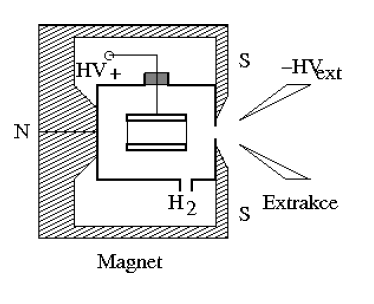
\includegraphics[width=0.6\textwidth]{vyboj.png}
		\captionof{figure}{Výbojový zdroj protonů PIG}		
	\end{center}
	
	\item INJEKCE ČÁSTIC DO STORAGE RINGU 
	
	Částice vyrobené ve zdroji a předurychlené lineárním urychlovačem je třeba vstříknout do synchrotronu, který je dále urychlí. To lze provést buď pomocí pulsních magnetů nebo - ve speciálních případech - pomocí vstřikování přes stripping folii. Díky urychlovacím vysokofrekvenčním dutinám může být na obvodu synchrotronu umístěno pouze určité množství shluků částic. Pokud jsou všechny tyto pozice zaplněny shluky částic na ose svazku, nelze již na osu svazku další shluky přidat. V této souvislosti mluvíme o zaplněném podélném fázovém prostoru urychlovače.
	
	 \begin{center}
		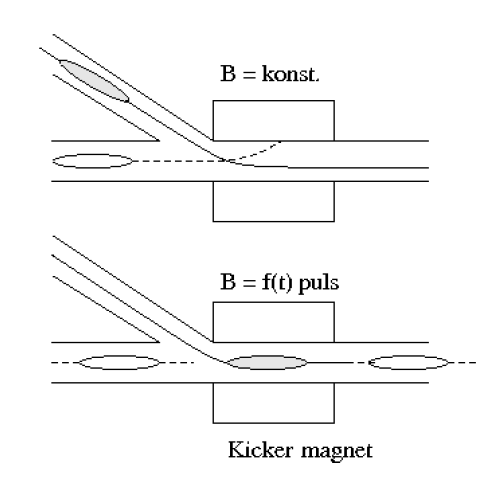
\includegraphics[width=0.6\textwidth]{injekce.png}
		\captionof{figure}{Injekce částic do urychlovače, zaplňování podélného fázového prostoru}		
	\end{center}
	
	Kdybychom pro navedení shluku na dráhu v synchrotronu použili magnet s konstantní magnetickou indukcí, došlo by k tomu, že vstřikovaný shluk by se sice dostal na správnou dráhu, ale shluky v urychlovači již cirkulující by z ní byly vychýleny a dopadly by na stěnu svazkové trubice. Pomocí pulsního magnetického pole působícího pouze v době průletu vstřikovaného shluku se tomuto problému můžeme vyhnout.
	
	Pokud potřebujeme přidat do synchrotronu další shluky částic, můžeme využít i příčný fázový prostor, do kterého lze umístit několik shluků mimo osu svazku. 
	
    \begin{center}
   	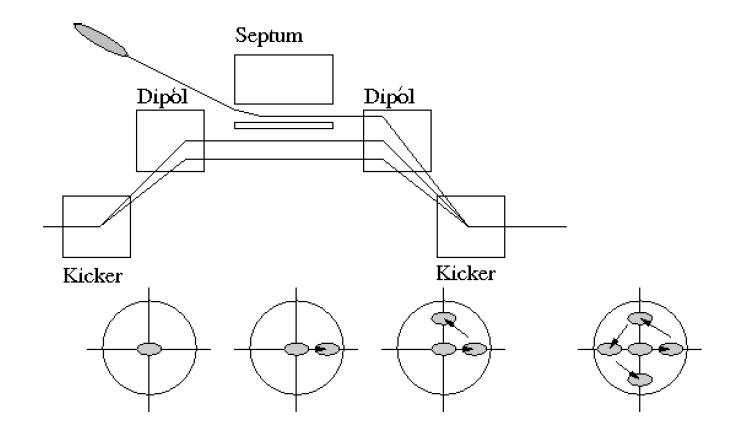
\includegraphics[width=0.7\textwidth]{plneni.png}
   	\captionof{figure}{Plnění příčného fázového prostoru urychlovače}		
   \end{center}

	\item INJEKCE PROTONŮ SKRZE STRIPPING FÓLII 
	
	Protony lze injektovat pomocí stripping folie. Negativní vodíkové ionty $H^-$ jsou vstříknuty do konstantního dipólového magnetického pole, které je v našem příkladu na obrázku zatáčí doleva. Po průletu stripping fólií jsou odtrženy oba elektrony a dále pokračuje pouze kladný proton. Po oběhu synchrotronu se proton dostává do pole prvního magnetu, který jej - díky kladnému náboji - zatáčí doprava a dopraví jej na stejnou dráhu jako vstřikovaný iont.
	
	\begin{center}
		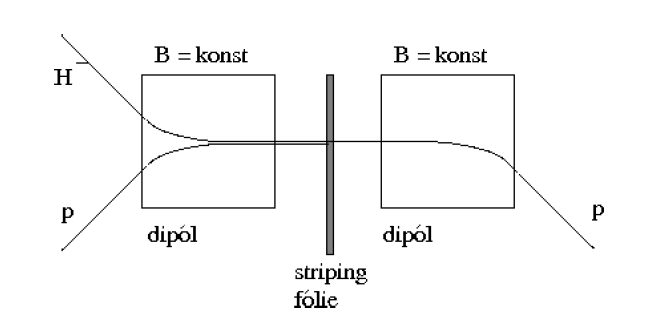
\includegraphics[width=0.7\textwidth]{stripp.png}
		\captionof{figure}{Plnění urychlovače přes stripping fólii}		
	\end{center}
	
	\item ELEKTRONIKA KICKERU 
	
	Nnyí si ukážeme schéma vinutí a elektroniky pulsního magnetu - kickeru. Aby bylo možno dosáhnout minimální délky pulsu, je třeba, aby vinutí kickeru mělo minimální indukčnost. Toho lze docílit způsobem vinutí , které je na obrázku vpravo. Pulsní proud se v cívce magnetu tvoří vybitím kondenzátoru přes sepnutou elektronku, na obrázku vlevo.
	
	Obvykle potřebujeme pulsy o délce $\approx 1 ~\mathrm{\mu s}$. Pro zobrazené vinutí můžeme indukci magnetického pole vypočíst ze vztahu
	\begin{equation}
	B_z = \dfrac{4 \mu_0 b}{\pi (a^2 + b^2)} I,
	\end{equation}
	kde $I$ je proud tekoucí vinutím, $\mu_0$ je permeabilita vakua, $a,b$ jsou rozměry vinutí.
	
	\begin{center}
		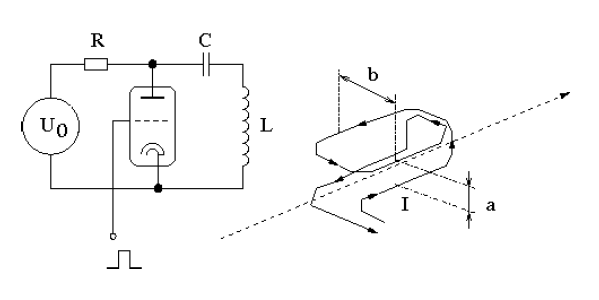
\includegraphics[width=0.9\textwidth]{kicker.png}
		\captionof{figure}{Geometrické uspořádání a elektronika kickeru}		
	\end{center}
	
\end{itemize}

\end{document}